\scanpage{26}
\mspage{7}
\figure{
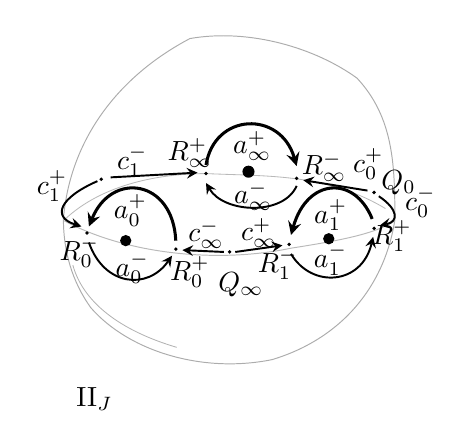
\begin{tikzpicture}[x=.012cm,y=-.012cm,>=stealth]
\draw[gray!65,line width=.35pt] (103,274)
 .. controls (110,190) and (161,123) .. (237,83)
 .. controls (300,72) and (370,93) .. (414,125)
 .. controls (453,167) and (454,218) .. (454,275)
 .. controls (443,346) and (397,401) .. (324,423)
 .. controls (250,438) and (172,414) .. (132,368)
 .. controls (112,340) and (103,308) .. (103,274);
\draw[gray!55,line width=.3pt] (104,275)
 .. controls (145,236) and (208,226) .. (254,226)
 .. controls (322,229) and (382,226) .. (444,263);
\draw[gray!55,line width=.35pt] (104,276)
 .. controls (171,312) and (268,321) .. (344,305)
 .. controls (395,297) and (433,290) .. (454,276);
\draw[gray!60,line width=.3pt] (113,323)
 .. controls (125,366) and (169,394) .. (223,410);
\coordinate (A) at (254,226); \coordinate (B) at (350,231);
\coordinate (C) at (128,289); \coordinate (D) at (222,306);
\coordinate (E) at (342,301); \coordinate (F) at (432,284);
\coordinate (U) at (143,232); \coordinate (V) at (432,246);
\coordinate (W) at (279,309);
\foreach \p in {A,B,C,D,E,F,U,V,W}{\fill (\p) circle (2.0);}
\fill (299,224) circle (6.4);
\fill (169,297) circle (6.0);
\fill (384,295) circle (6.0);
\draw[->,line width=1.1pt] (254,217)
 .. controls (263,161) and (333,159) .. (350,218);
\draw[->,line width=.7pt] (350,239)
 .. controls (336,271) and (273,268) .. (254,236);
\draw[->,line width=1.1pt] (222,297)
 .. controls (219,232) and (154,223) .. (130,282);
\draw[->,line width=.7pt] (130,299)
 .. controls (146,345) and (192,350) .. (218,313);
\draw[->,line width=1.1pt] (430,274)
 .. controls (411,227) and (361,231) .. (344,291);
\draw[->,line width=.7pt] (344,311)
 .. controls (366,348) and (419,344) .. (431,293);
\draw[->,line width=.7pt] (139,234)
 .. controls (98,252) and (91,272) .. (122,282);
\draw[->,line width=.7pt] (153,230)--(245,225);
\draw[->,line width=.7pt] (425,244)--(357,233);
\draw[->,line width=.7pt] (437,250)
 .. controls (458,264) and (458,277) .. (438,281);
\draw[->,line width=.7pt] (273,309)--(229,307);
\draw[->,line width=.7pt] (285,309)--(335,302);
\node at (303,197) {$a_\infty^+$};
\node at (304,250) {$a_\infty^-$};
\node at (174,265) {$a_0^+$};
\node at (176,326) {$a_0^-$};
\node at (386,270) {$a_1^+$};
\node at (386,317) {$a_1^-$};
\node at (91,239) {$c_1^+$};
\node at (176,213) {$c_1^-$};
\node at (426,216) {$c_0^+$};
\node at (481,256) {$c_0^-$};
\node at (254,290) {$c_\infty^-$};
\node at (310,289) {$c_\infty^+$};
\node at (237,204) {$R_\infty^+$};
\node at (379,219) {$R_\infty^-$};
\node at (120,309) {$R_0^-$};
\node at (237,330) {$R_0^+$};
\node at (330,322) {$R_1^-$};
\node at (451,292) {$R_1^+$};
\node at (458,236) {$Q_0$};
\node at (291,344) {$Q_\infty$};
\node at (136,465) {$\mathrm{II}_J$};
\end{tikzpicture}
}
On rajoute les sommets $Q_i$ $(i\in J)$ et les arcs
\diagram{\begin{tikzcd}[ampersand replacement=\&]Q_i\arrow[r,"c_i^\omega"]\&R_{\omega'i}^{\omega'}\end{tikzcd}}
permutés \inserted{de façon \unsure{simple|simplement}}
\unsure{transitive}\deleted{\unsure{ment}} par $G_J$. On a maintenant
\[
(13)\qquad b_i^\omega=c_i^\omega(c_i^{\omega'})^{-1}
\]
(donc les $b_i^\omega$ deviennent inutiles comme générateurs d'un groupoïde).
\inserted{Dans} Les relations \inserted{$(2)$} \deleted{deviennent},
la partie $(a)$ devient automatique, pour écrire commodément la partie $(b)$,
on introduit les
\[
(14)\qquad\widetilde a_i^\omega=
\begin{gathered}
(\unsure{c}_{\unsure{\omega i|\omega'i}}^{\omega\deleted{\unsure{'}}})^{-1}
a_i^{\omega\deleted{\unsure{'}}}
\unsure{c}_{\unsure{\omega'i|\omega i}}^{\omega'}\\[-2pt]
\inserted{(c_{\omega i}^\omega)^{-1}a_i^\omega c_{\omega'i}^{\omega'}}
\end{gathered}
:\quad Q_{\omega'i}\longrightarrow Q_{\omega i}
\]
\figure{
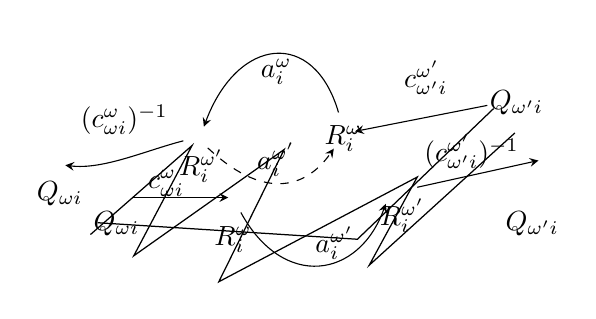
\begin{tikzpicture}[x=1cm,y=1cm,>=stealth]
\node (qu) at (0,0) {$Q_{\omega i}$};
\node (rl) at (1.8,.35) {$\unsure{R_i^{\omega'}}$};
\node (rr) at (3.6,.7) {$R_i^\omega$};
\node (qr) at (5.8,1.15) {$Q_{\omega'i}$};
\draw[->] (1.57,.67) .. controls (1.1,.55) and (.55,.3) .. (.07,.36);
\node at (.82,.94) {$(c_{\omega i}^\omega)^{-1}$};
\draw[->] (5.43,1.12)--(3.75,.79);
\node at (4.65,1.47) {$c_{\omega'i}^{\omega'}$};
\draw[->] (3.54,1.03) .. controls (3.23,2.1) and (2.26,2.0) .. (1.83,.85);
\node at (2.75,1.55) {$a_i^\omega$};
\draw[->,dashed] (1.88,.58) .. controls (2.56,-.06) and (3.1,.03) .. (3.48,.57);
\node at (2.75,.43) {$a_i^{\omega'}$};
\node at (.72,-.38) {$\deleted{\unsure{Q_{\omega i}}}$};
\node at (2.2,-.58) {$\deleted{\unsure{R_i^\omega}}$};
\node at (4.35,-.28) {$\deleted{\unsure{R_i^{\omega'}}}$};
\node at (6.0,-.38) {$\deleted{\unsure{Q_{\omega'i}}}$};
\draw[->] (.92,-.05)--(2.14,-.05);
\node at (1.35,.13) {$\deleted{\unsure{c_{\omega i}^\omega}}$};
\draw[->] (2.3,-.24) .. controls (2.84,-1.23) and (3.8,-1.08) .. (4.14,-.13);
\node at (3.49,-.63) {$\deleted{\unsure{a_i^{\omega'}}}$};
\draw[->] (4.54,.08)--(6.08,.42);
\node at (5.23,.53) {$\deleted{(c_{\omega'i}^{\omega'})^{-1}}$};
\draw[line width=.45pt] (.39,-.52)--(1.68,.61)--(.94,-.79)--(2.85,.56)
 --(2.02,-1.12)--(4.54,.21)--(3.93,-.91)--(5.78,.77);
\draw[line width=.45pt] (.48,-.37)--(3.78,-.58)--(5.51,1.08);
\end{tikzpicture}}
\margin{\figure{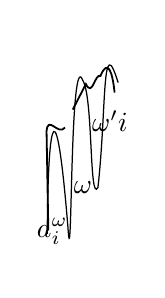
\begin{tikzpicture}[x=.45cm,y=.6cm]
\draw[line width=.45pt] (.05,.15) .. controls (.07,2.8) and (.32,3.28) .. (.65,.13)
 .. controls (.75,-.6) and (.7,4.1) .. (1.05,3.4)
 .. controls (1.35,3.05) and (1.23,.78) .. (1.48,1.13)
 .. controls (1.73,2.8) and (1.58,4.5) .. (2.05,3.35);
\draw[line width=.65pt] (.08,.22)--(.03,2.32)
 .. controls (.07,2.68) and (.36,2.21) .. (.55,2.4);
\draw[line width=.65pt] (.77,2.78)--(1.14,3.32)
 .. controls (1.33,3.03) and (1.39,3.55) .. (1.55,3.49)
 .. controls (1.76,3.87) and (1.89,3.58) .. (1.95,3.14);
\node at(.19,.2){$\unsure{a_i^\omega}$};
\node at(1.06,1.13){$\unsure{\omega}$};
\node at(1.82,2.53){$\unsure{\omega'i}$};
\end{tikzpicture}}}
qui sont également permutés de façon simpl. transitive sous $G_J$, et on a
\[
(15)\qquad\tau(\widetilde a_i^\omega)=(\widetilde a_i^{\omega'})^{-1}
\]
La relation $(2b)$ devient
\[
(16)\qquad\widetilde a_{\omega^2i}^\omega\widetilde a_{\omega i}^\omega\widetilde a_i^\omega=1
\]
(deux relations ess\textsuperscript{t}. distinctes\unsure{,} qui sont permutées par $\tau$)

Pour repérer les \inserted{$\pi(Q_{\unsure{J|i}})=$}
$\pi_1(\Sigma_J(\mathbb C),Q_i)$ de façon commode on utilise les
\diagram{
\begin{tikzcd}[ampersand replacement=\&,column sep=large,row sep=large]
(17)\quad\psi_i^\omega:\ \deleted{Q_i}\Pi_{0,3}
\arrow[rr,"\sim"]
\arrow[dr,"\varphi_{\omega'i}^{\omega'}","\sim"',sloped]
\&\&\pi(Q_i)\\
\&\pi(R_{\omega'i}^{\omega'})
\arrow[ur,"(c_i^\omega)^{-1}"',"\sim",sloped]
\arrow[ur,phantom,near end,"\deleted{\unsure{c|\sim}}"]\&
\end{tikzcd}}
\margin{\uline{NB}\quad$\tau\psi_i^\omega(g)=\psi_i^\omega(\tau_\infty g)$}
on aura
\[
(18)\qquad\psi_i^\omega(g)=\psi_i^{\omega'}(\sigma_\infty(g))
\]
\[
(19)\qquad\begin{aligned}
\widetilde a_i^{\omega\deleted{\unsure{'|*}}}
(\psi_{\omega'i}^{\omega'}(g))
&=\psi_{\omega\deleted{\unsure{'}}i}^{\omega\deleted{\unsure{'}}}
(\varepsilon_0(g))
=\psi_{\omega\deleted{\unsure{'}}i}^{\omega'}
(\overbrace{\sigma_\infty\varepsilon_0}^{\deleted{\unsure{\xi|\rho}}=\tau_\infty(\rho)}(g))
\end{aligned}
\]
\[
\begin{array}{|c|}\hline
\displaystyle \widetilde a_i^\omega(\psi_{\omega'i}^{\omega}(g))
=\psi_{\omega\deleted{\unsure{'}}i}^{\omega\deleted{\unsure{'}}}
(\overbrace{\varepsilon_0\deleted{\unsure{(}}\sigma_\infty}^{\rho^{-1}})(g))\\
\end{array}
=\psi_{\omega'i}^{\omega'}(\sigma_\infty\varepsilon_0\sigma_\infty(g))
\]
\margin{25}
